\chapter{CASE STUDIES}
\label{caseStudyChapter}
In this section two case studies are examined. The first is the 2011 Chinese drought and the second is a simulated future event where the United States corn exports are reduced. The first case study shows the basic use of the system and shows how we can identify vulnerable countries based on simulated climate events. Although the first case study does not highlight the cascading effects it does show that the vulnerability of a country may be affected by the simulation of a climate event. In our second case study we explore a full use case scenario of the system by targeting one of the largest corn exporters, the United States, and simulating a moderate climate event. In doing so we highlight the cascading effects to the food trade network and visualize the potentially vulnerable countries affected by a simulated climate event.\par
\section{2011 Chinese Drought}
In 2011 the United Nations’ food agency issued an alert warning that a severe drought was threatening the wheat crop in China, the world's largest wheat producer, and resulting in shortages of drinking water for people and livestock \citep{bradsher2011food}. In response to the drought China was forced to import more wheat instead of relying on its self sufficiency as in previous years \citep{sternberg2012chinese}. The increase in demand drives the price of wheat up as show in Table \ref{wheatTable}. This coupled with a number of countries implementing export bans the previous year \citep{fellmann2014harvest} has a great potential for a disrupted food trade network.\par
\begin{center}
	\begin{table}[htb]
		\centering
		\begin{tabular}{| c | c | c | c |}
			\hline
			Country & Market Year & Wheat Price USD / Ton & Exported to China (million USD)\\
			\hline \hline
			Australia & 2010 & \$200.00 & \$179\\ \hline
			Australia & 2011 & \$265.10 & \$180\\ \hline
			Australia & 2012 & \$235.00 & \$628\\ \hline
			Australia & 2013 & \$302.20 & \$242\\ \hline \hline
			Canada & 2010 & \$177.10 & \$72\\ \hline
			Canada & 2011 & \$237.00 & \$63\\ \hline
			Canada & 2012 & \$253.90 & \$163\\ \hline
			Canada & 2013 & \$252.90 & \$300\\ \hline \hline
			USA & 2010 & \$209.00 & \$36\\ \hline
			USA & 2011 & \$266.00 & \$159\\ \hline
			USA & 2012 & \$286.00 & \$224\\ \hline
			USA & 2013 & \$252.00 & \$1,292\\ \hline
		\end{tabular}
		\caption[WHEAT PRICE DATA FOR YEARS 2010 - 2013]{Wheat price data for years 2010 - 2013 (FAOSTAT Producer Prices - Annual) \citep{faostat}}
		\label{wheatTable}
	\end{table}
\end{center}
Halfway around the world in Egypt, the world's largest importer of wheat, was the resonance felt; wheat prices doubled the price of bread tripled \citep{sternberg2012chinese}. According to \cite{croppenstedt2006food} bread provides around one-third of the daily Egyptian caloric intake. These two factors prompted bread shortages and price increases in parts of the country that contributed to bread-inspired demonstrations and directly influenced political protest. \par
During this time many export restrictions were in place, including Russia's export ban \citep{fellmann2014harvest}. For simulation purposes, we model this export ban a 100\% export reduction out of Russia and run the simulation to see the vulnerable countries. Modeling it in this way allows us to see a number of countries significantly affected by the ban. Among them is Egypt, as anticipated, displaying an almost 40\% loss of imports (Figure \ref{egypt2011}, tooltip). From the red coloring in the choropleth map (Figure \ref{egypt2011}), the visual analytic system marks this as a potential area of vulnerability. Examining the network graph by filtering for very large links (great than \$500 million), Figure \ref{egypt2011-2013}-1 shows Egyptian imports of wheat from their main providers. In 2011 Egypt imports over \$2 billion from the United States and Russia. In 2013 that number is reduced to just \$1.1 billion. Though I make no claims of correlation, the 40\% reduction postulated from the simulation mirrors what is seen in Figure \ref{egypt2011-2013}.\par
\begin{figure}[htb]
	\center{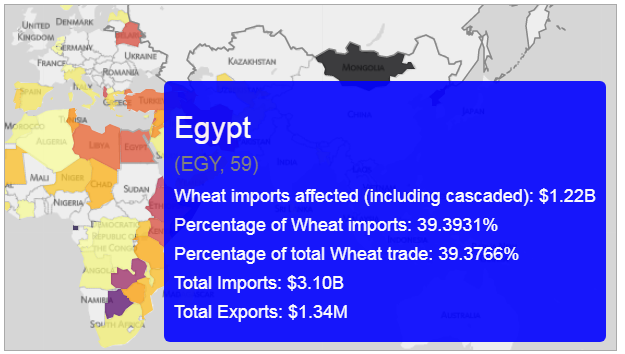
\includegraphics[width=\textwidth]{figures/egypt2011.png}}
	\caption[CHOROPLETH MAP OF SIMULATED RUSSIAN WHEAT EXPORT BAN]{Choropleth map of simulated Russian wheat export ban. The red color indicates that Egypt is moderately vulnerable to a climate event forcing an export reduction from Russia. The tooltip shows that Egypt would lose about \$1.22 billion in wheat imports accounting for almost 40\% of their entire import of wheat.}
	\label{egypt2011}
\end{figure}
Another aspect of analyzing the 2011 Chinese drought is supported by the system is exploration of the temporal changes to the food trade network by visualizing the graph year over year, as in Figure \ref{china2010-2013}, to look for patterns. We expect that there will be changes to the food trade network because of the aforementioned 2011 Chinese drought. The views in Figure \ref{china2010-2013} are set by selecting the first year to examine, 2010, and then filtered the network graph to only show links of greater than \$50 million. Each successive view only the year was modified.\par
As expected, looking at the graph we notice this sharp increase in imports of wheat to China. In 2010 China is largely self-sufficient; with imports of only \$296 million (Figure \ref{china2010-2013}-1, tooltip). In 2011 and 2012 we see still more increases in imports. Finally, moving to 2013, Chinese imports of wheat increased to \$1.90 billion (Figure \ref{china2010-2013}-4, tooltip), an increase of 640\%. The links go from virtually non-existent (figure \ref{china2010-2013}-1 US to China, \$56M in 2010, link not visible) to a trade link that is of a significant value (Figure \ref{china2010-2013}, bottom left; US to China, \$1.292 billion in 2013, large blue line). Moreover, from this progression we see the shift from Chinese self-sufficiency to import dependency.\par
From this case study we have demonstrated that our visual analytic system can help analysts explore the impacts of historical climate events on the international food trade network. 
\begin{figure}[htb]
	\center{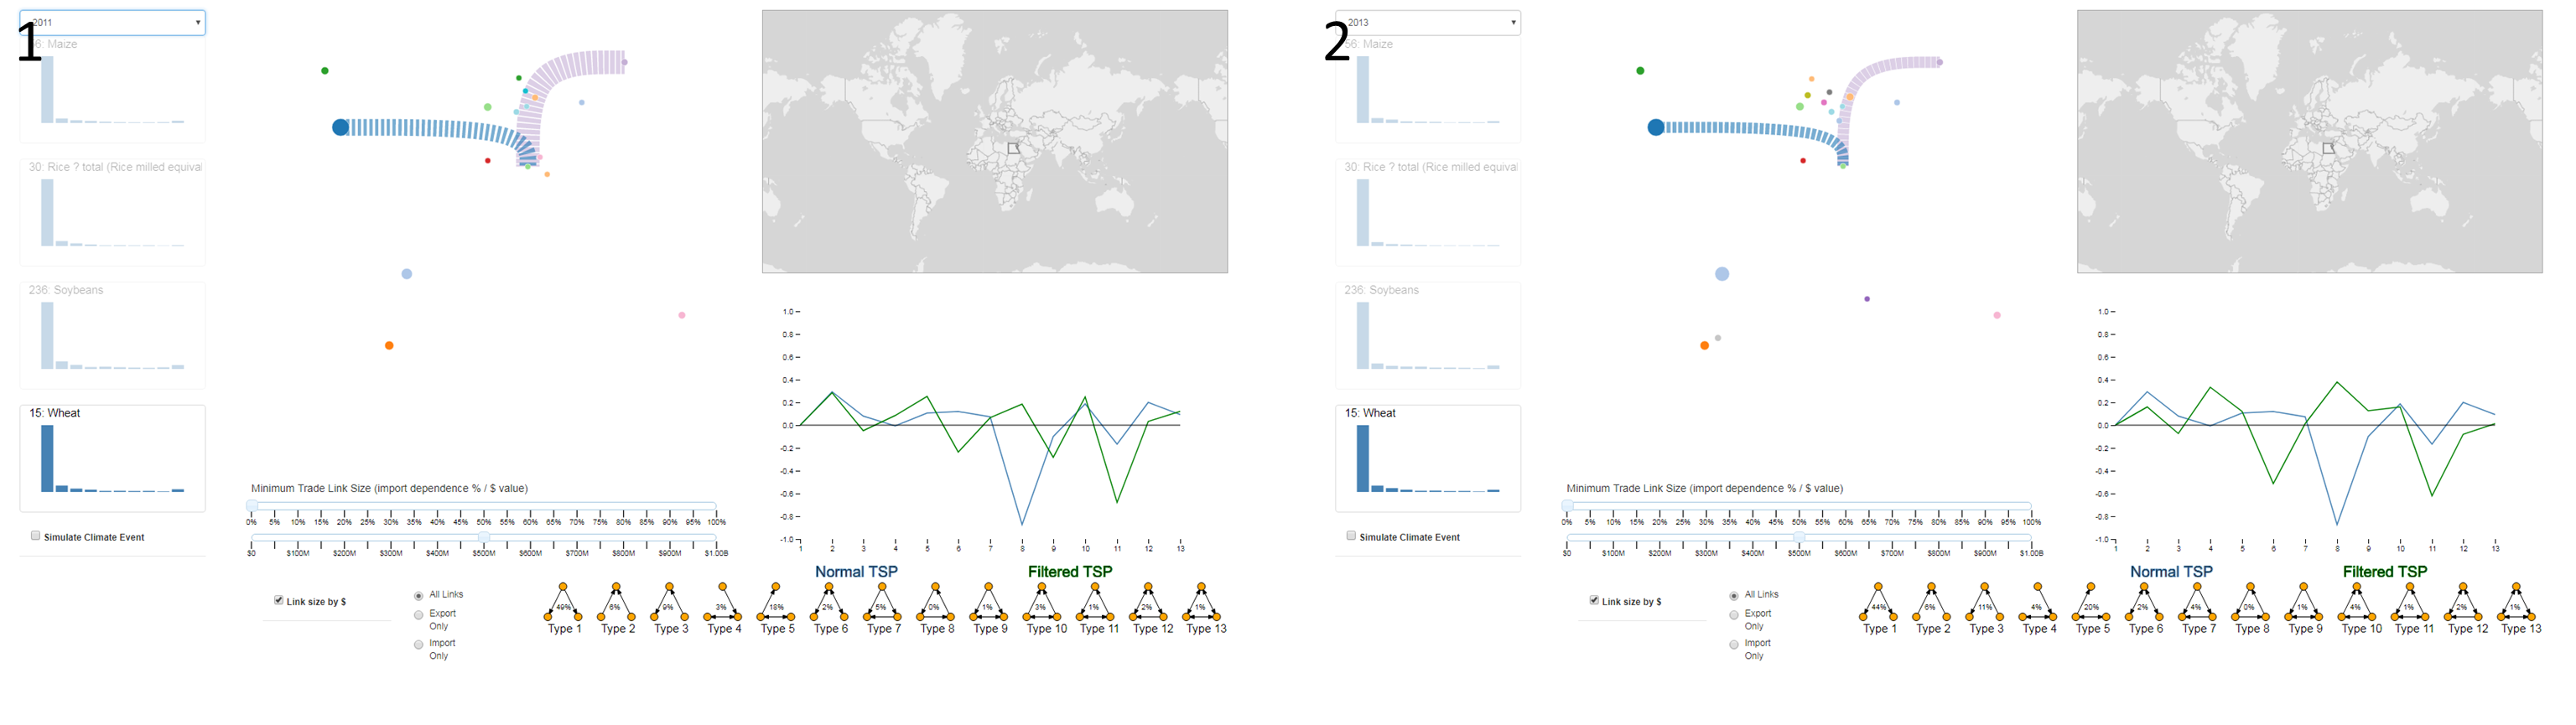
\includegraphics[width=\textwidth]{figures/egypt2011-2013.png}}
	\caption[PROGRESSION OF EGYPT WHEAT IMPORTS FROM 2011 TO 2013]{Left: {In 2011 Egypt (light blue) imports \$852 million in wheat from the United States (dark blue) and \$1.219 billion from Russia (pink). A total of approximately \$2.071 billion}; Right: {In 2013 Egypt (light blue) imports \$558 million in wheat from the United States (dark blue) and \$576 million from Russia (pink). A total of approximately \$1.134 billion is close to half of the value imported just two years ago.}}
	\label{egypt2011-2013}
\end{figure}
\begin{figure}[htb]
	\center{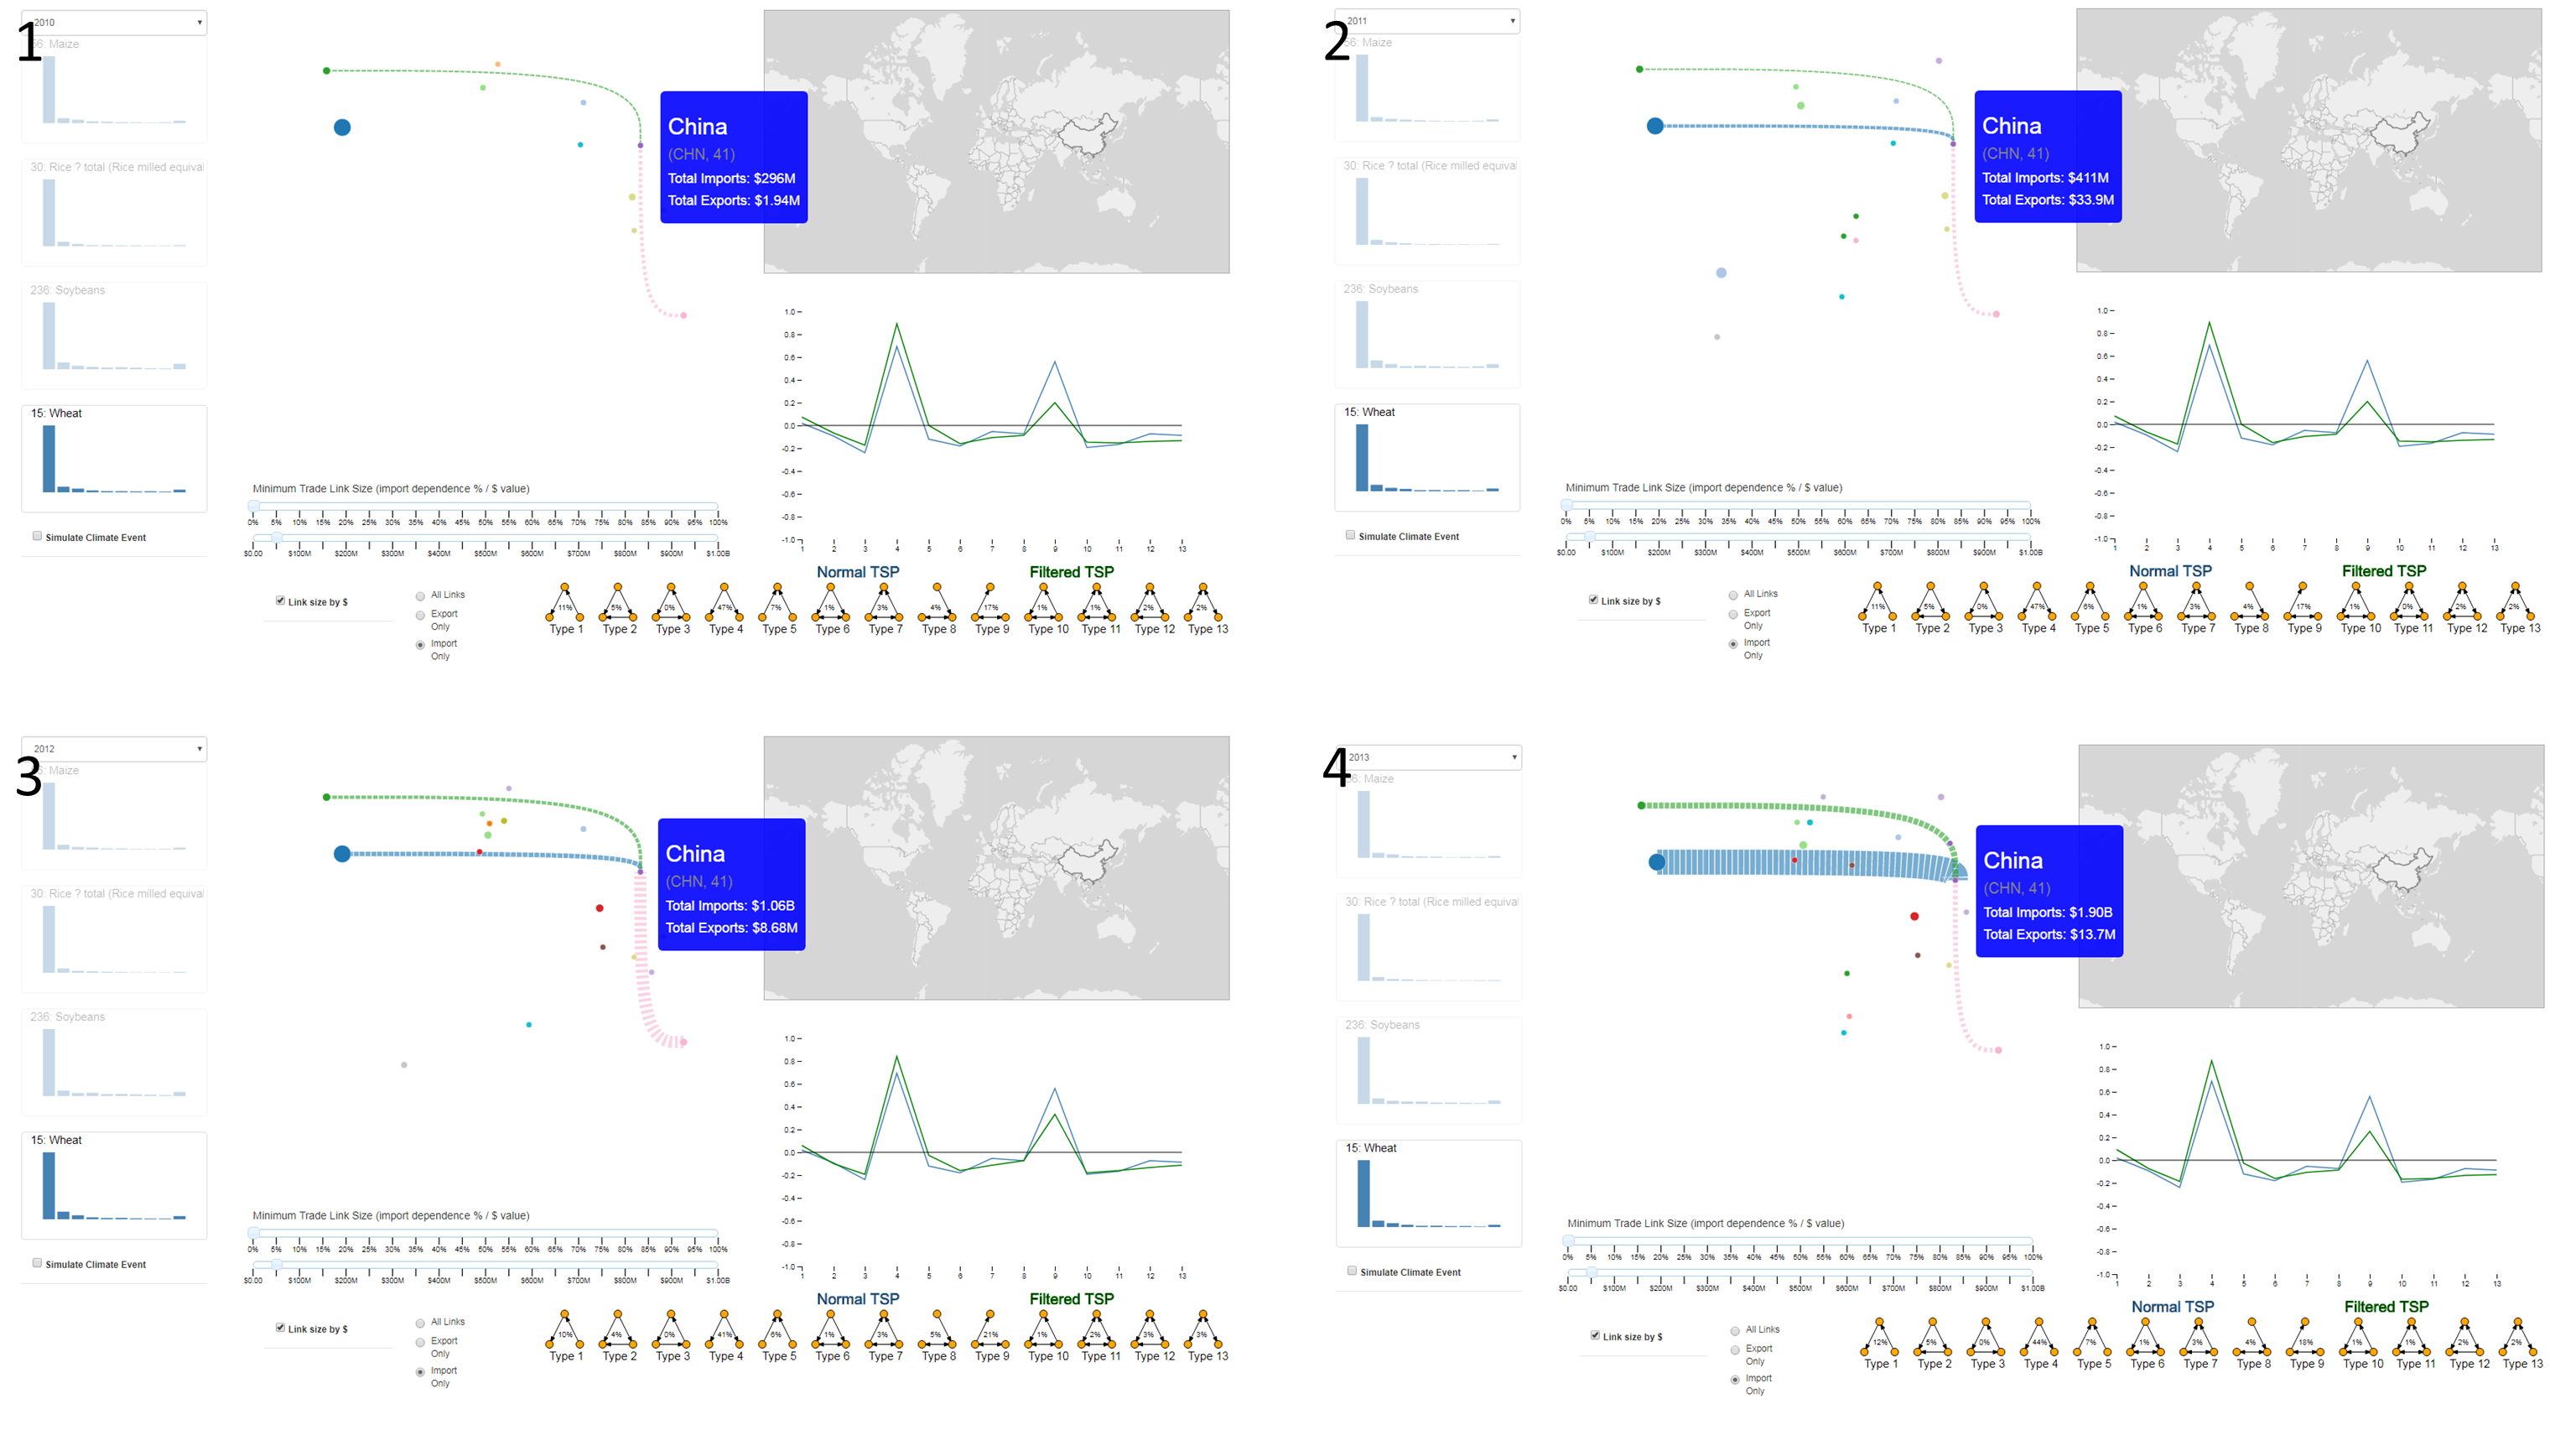
\includegraphics[width=\textwidth]{figures/china.png}}
	\caption[PROGRESSION OF SIGNIFICANT CHINESE WHEAT IMPORTS FROM 2010 TO 2013]{Progression of significant Chinese wheat imports from 2010 to 2013. Top Left: {In 2010 China (purple) imported \$36 million in wheat from the United States (blue, link not shown), \$72 million from Canada (green) and \$179 million from Australia (pink). From the tooltip China imported a total \$296 million}; Top Right: {In 2011, during the first year of the crisis, China (purple) imported \$159 million in wheat from the United States (blue), \$63 million from Canada (green) and \$180 million from Australia (pink). From the tooltip China imported a total \$411 million}; Bottom Left: {By 2012, with a sharp increase in imports directly related to the drought, China (purple) imported \$224 million in wheat from the United States (blue), \$163 million from Canada (green) and \$628 million from Australia (pink). From the tooltip China imported a total \$1.06 billion, almost four times the amount in 2010.}; Bottom Right: {By 2013 China (purple) being increasingly dependent on the \$1.292 billion imported from the United States (blue), \$300 million from Canada (green) and \$242 million from Australia (pink). From the tooltip China imported a total \$1.90 billion, a more than six-fold increase from 2010. }}
	\label{china2010-2013}
\end{figure}
\clearpage
\section{Simulated 2020 US Climate Event}
As a second case study, we will use the system to simulate the effect of an unspecified climate event to the United States. As a demonstration we will highlight the downstream effects of a major reduction in exports of corn from the United States.\par
Although the United States was chosen a priori, we could have used the 2013 trade data as a starting point to start the selection process for a country. This can be done by first inspecting the histograms. The tooltip in Figure \ref{cs2-0} shows three major importers, in both dollar value and import dependency, of United States' exports of corn: Mexico at \$1.85 billion and 92\%, China at \$1.05 billion and 91\% and Canada at \$281 million and 94\%. However, as import dependency is a function of the export value as well (Equation \ref{vulnerability}) we confirm import dependency on the network graph. To do so we filter the network graph to show only countries with an import dependence of at least 75\% and trade link values of at least \$100 million (Figure \ref{cs2-0}, sliders). Note that in this instance we could have filtered the network graph first, but using the histograms allows for the inspection of smaller countries. We do see two of the identified links still present (Figure \ref{cs2-0}, the two blue lines) with this filtering (the United States to Mexico and the United States to China) and so we decide to continue the analysis with the United States as the selected country. As the United States is one of the major exporters of corn (\$6.98 billion in 2013 according to the tooltip in Figure \ref{cs2-1}-1), we expect to see a number of vulnerable countries, even ones with no direct trade links with the United States. A 15\% export reduction is chosen arbitrarily as a starting point.\par
\begin{figure}[htb]
	\center{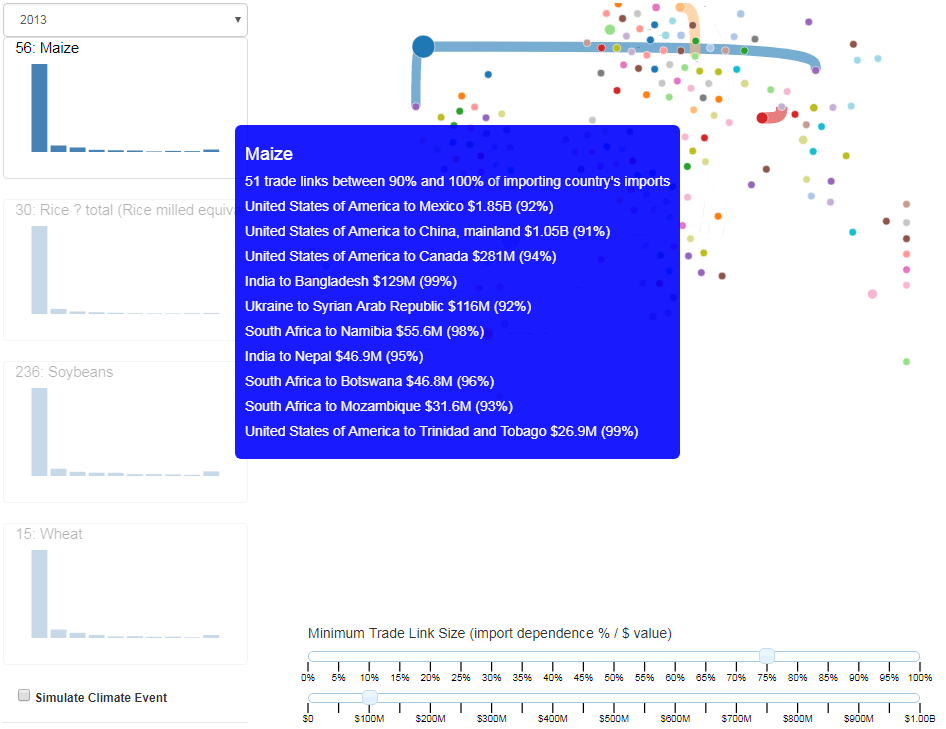
\includegraphics[width=\textwidth]{figures/selecting.png}}
	\caption[PROCESS OF SELECTING A COUNTRY FOR THE SIMULATION]{The process of selecting a country for the simulation starts with looking at the histograms and confirming on the network graph. Here the tooltip for the histogram displays the name of exporting and importing country along with the dollar value and import dependence of the trade link. This shows multiple potentially import dependent countries as indicated by a high import dependence percentage. The dependencies can be confirmed with filtering on the network graph (sliders on the bottom). The links remaining visible (the United States to Mexico, the United States to China, India to Bangladesh and Ukraine to the Syria Arab Republic) coincide with the histogram information.}
	\label{cs2-0}
\end{figure}
As the United States was chosen as a potential candidate for simulation, we select the node representing the United States (large blue node, approximately geographically positioned). The node and country in the map are drawn with dark borders to indicate it has been selected (Figure \ref{cs2-1}-1). As expected, and as shown in the network graph (Figure \ref{cs2-1}-1), there are a large number of countries involved in corn trade with the United States. Next the \textit{Simulate Climate Event} checkbox is selected and we select a 15\% reduction as shown in bottom left of Figure \ref{cs2-1}-2. The network graph in Figure \ref{cs2-1}-2 shows there are a large number of cascaded effects, represented by the now visible trade links. However, further filtering is required to gain context. In Figure \ref{cs2-1}-3 the \textit{Minimum Percentage of Imports Affected} is changed to 30\%. This filters the network graph to only display the links affecting those countries whose imports have been reduced by at least 30\%. Examining the choropleth map of the current state in Figure \ref{cs2-2}, we see that Venezuela, North Korea and Mongolia are affected heavily based on the darker coloring.\par
\begin{figure}[htb]
	\center{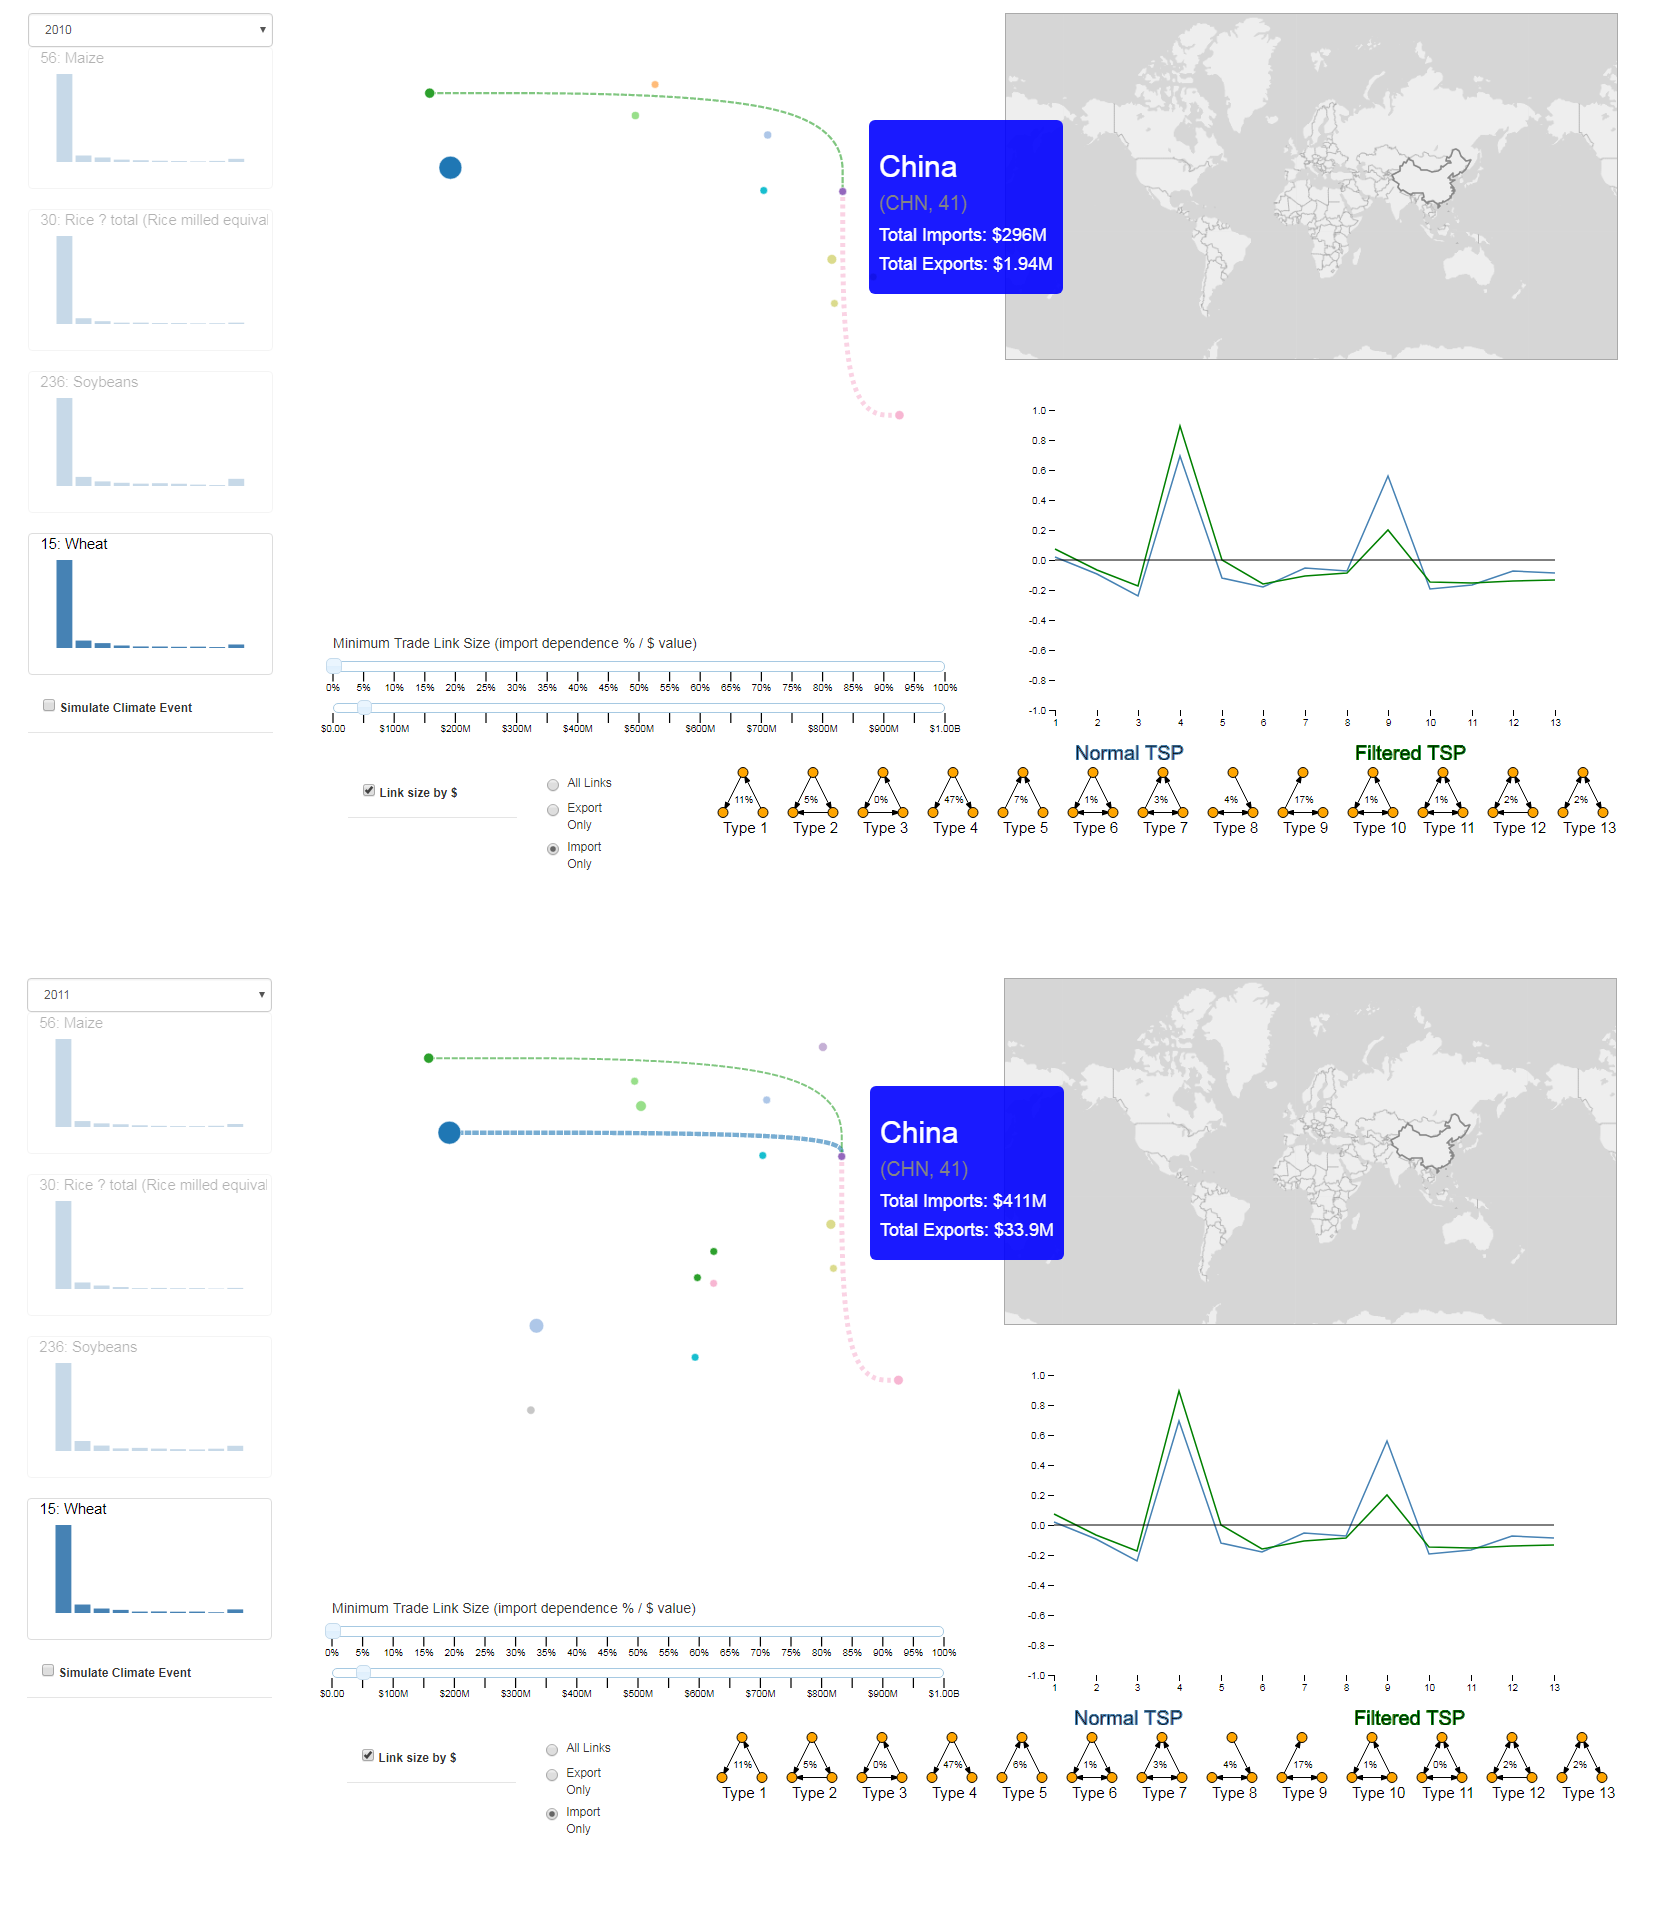
\includegraphics[width=\textwidth]{figures/cs2-1_tt.png}}
	\caption[RUNNING A SIMULATION AND EXPLORING RESULTS]{Running a simulation and exploring results. 1: {The United States is selected}; 2: {Simulation is ran with a 15\% export reduction from the United States}; 3: {Simulation results filtered on countries with import losses of at least 30\% and showing only links of at least a \$200 million dollar value}; 4: {Tooltip of the trade link from the United States to Venezuela} }
	\label{cs2-1}
\end{figure}
\begin{figure}[htb]
	\center{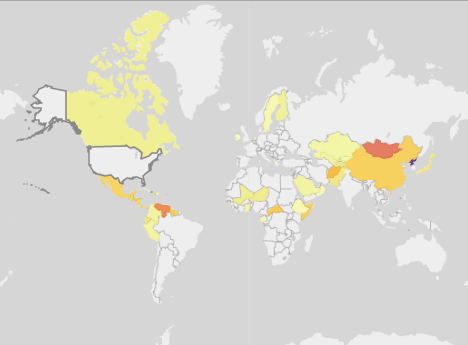
\includegraphics[width=\textwidth]{figures/cs2-2.png}}
	\caption[SIMULATION CHOROPLETH MAP]{A zoomed in view of the choropleth map from the simulation.}
	\label{cs2-2}
\end{figure}
To examine the impact on Venezuela we look at the trade links coming into Venezuela. The link from the United States shows a reduction of only \$55.5 million (Figure \ref{cs2-1}-4, tooltip), which is significantly less than the \$301 million shown in the country's information (Figure \ref{cs2-3}-1, tooltip). To look for other major import sources we slowly adjust the trade link size by dollar filter until only the top few links are shown (Figure \ref{cs2-3}-2, second slider has moved to \$200 million). Examining the link from Argentina to Venezuela (Figure \ref{cs2-3}-2, tooltip) shows a loss of only \$41k which has relatively little impact to the \$301 million loss. Examining the other link, Mexico to Venezuela, reveals the cascaded effect. Figure \ref{cs2-3}-4, tooltip, shows that Mexico's trade link to Venezuela has been reduced by \$240 million, a significant portion of the \$301 million total import loss to Venezuela. The export reduction of 15\% from the United States prompts a loss of \$280 million to Mexico (Figure \ref{cs2-3}-4) which is mostly passed on to Venezuela. Thus, Venezuela is indirectly impacted by a climate event to the United States, to the degree of approximately one third of their entire import of corn.\par
\begin{figure}[htb]
	\center{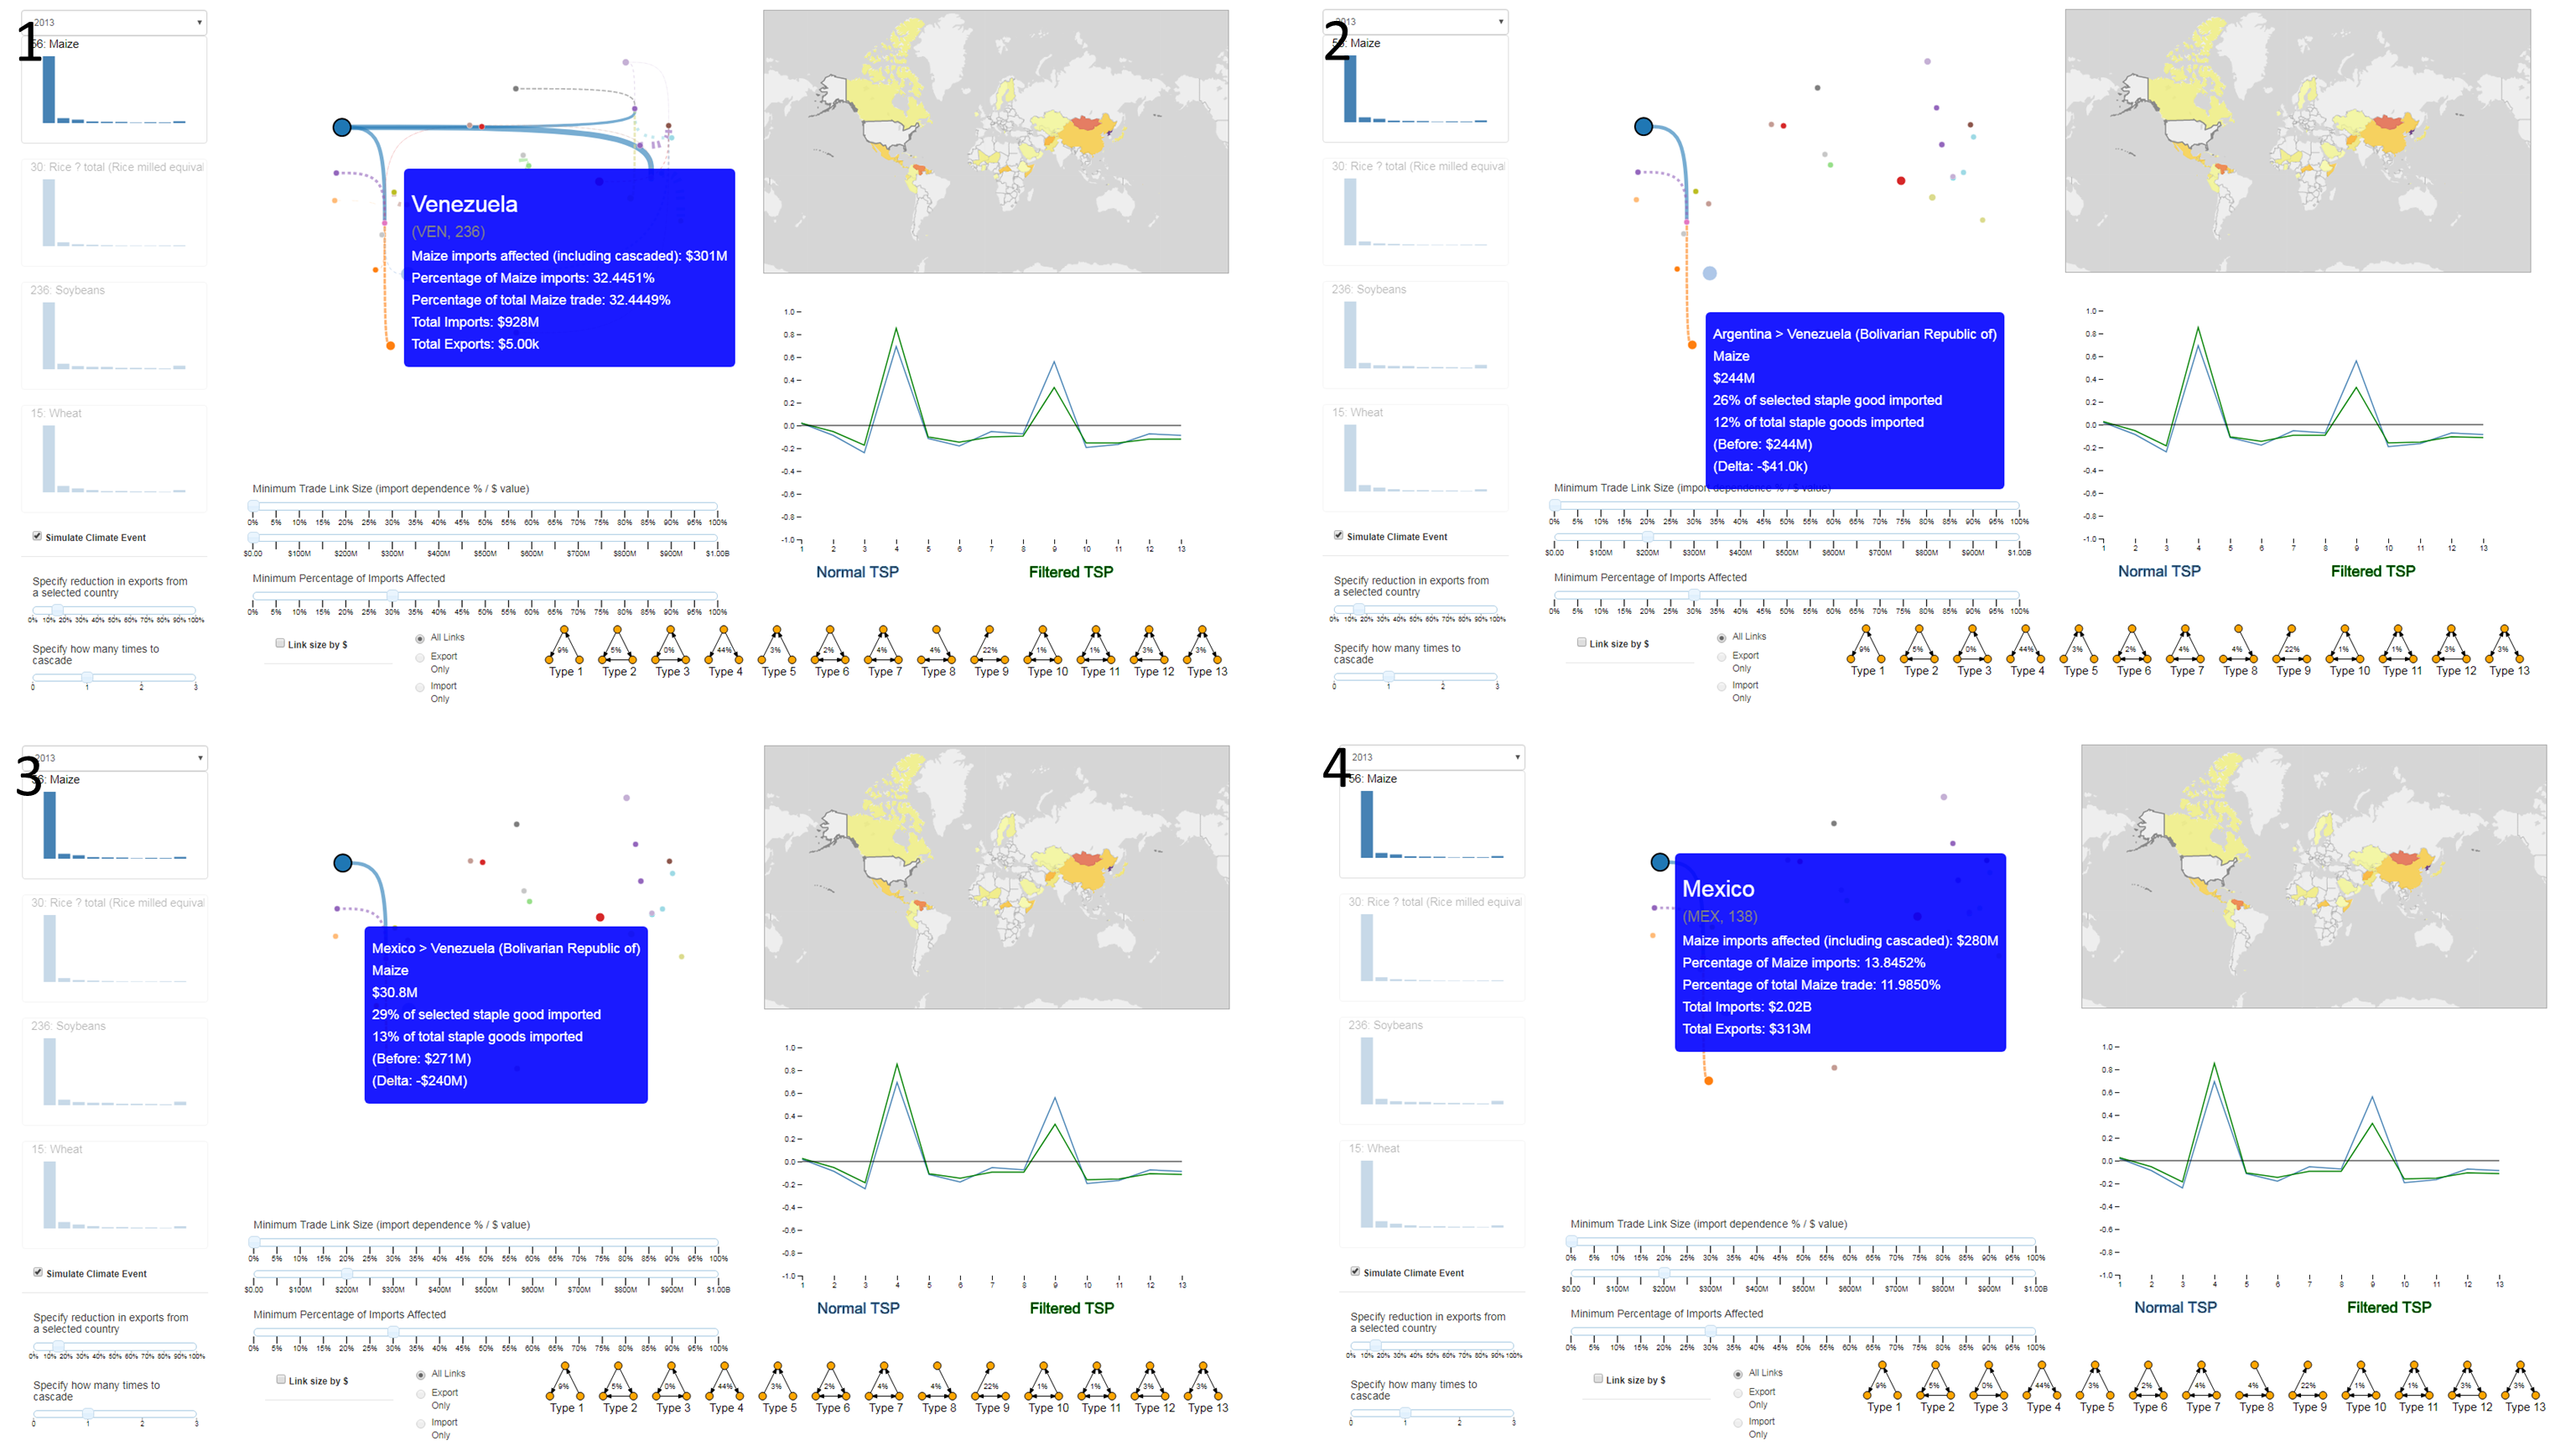
\includegraphics[width=\textwidth]{figures/cs2-3.png}}
	\caption[EXAMINING THE RESULTS OF A SIMULATION, FILTERED ON LARGE DOLLAR VALUE (\$200 MILLION) AND MODERATE IMPORT LOSSES (30\% LOSS)]{Examining the results of a simulation, filtered on large dollar value (\$200 million) and moderate import losses (30\% loss). 1: {Tooltip showing the impact to Venezuela}; 2: {Tooltip of the trade link from Argentina to Venezuela}; 3: {Tooltip of the trade link from Mexico to Venezuela}; 4: {Tooltip showing the impact to Mexico} }
	\label{cs2-3}
\end{figure}
Another example of use would be to see countries that are significantly (e.g. import losses of greater than 75\%) impacted by the climate event. We adjust the \textit{Minimum Percentage of Imports Affected} to 75\% (Figure \ref{cs2-4}-1) and \textit{Minimum Trade Link Size} to \$25 million to filter out the insignificant trade links. As indicated by the dark coloring in the choropleth map in Figure \ref{cs2-2}, the impact to North Korea is significant. However, no solid blue line (export from the United States) connects to North Korea (brown dot) in Figure \ref{cs2-4}-1 so no direct link exists from the United States to North Korea. Yet North Korea's imports are simulated to be affected by almost 80\% (Figure \ref{cs2-4}-2, tooltip). By examination of the link (Figure \ref{cs2-4}-3) we conclude that China acts as a middle man. The tooltip in Figure \ref{cs2-4}-4 shows that China lost imports of \$158 million. The same tooltip shows that it only exports \$34.2 million. Since the loss of imports is assumed to be first mitigated by reduction of exports, China essential breaks all export links to recoup the \$158 million loss of imports. This is a potential limitation of the system as China may still export the relatively small amount of \$31.9 million (Figure \ref{cs2-4}-3) to North Korea depending on a number of factors. (e.g. political repercussions, temporal considerations such as season). This example shows the cascading effect of the loss of imports to China from the United States being propagated to North Korea.\par
\begin{figure}[htb]
	\center{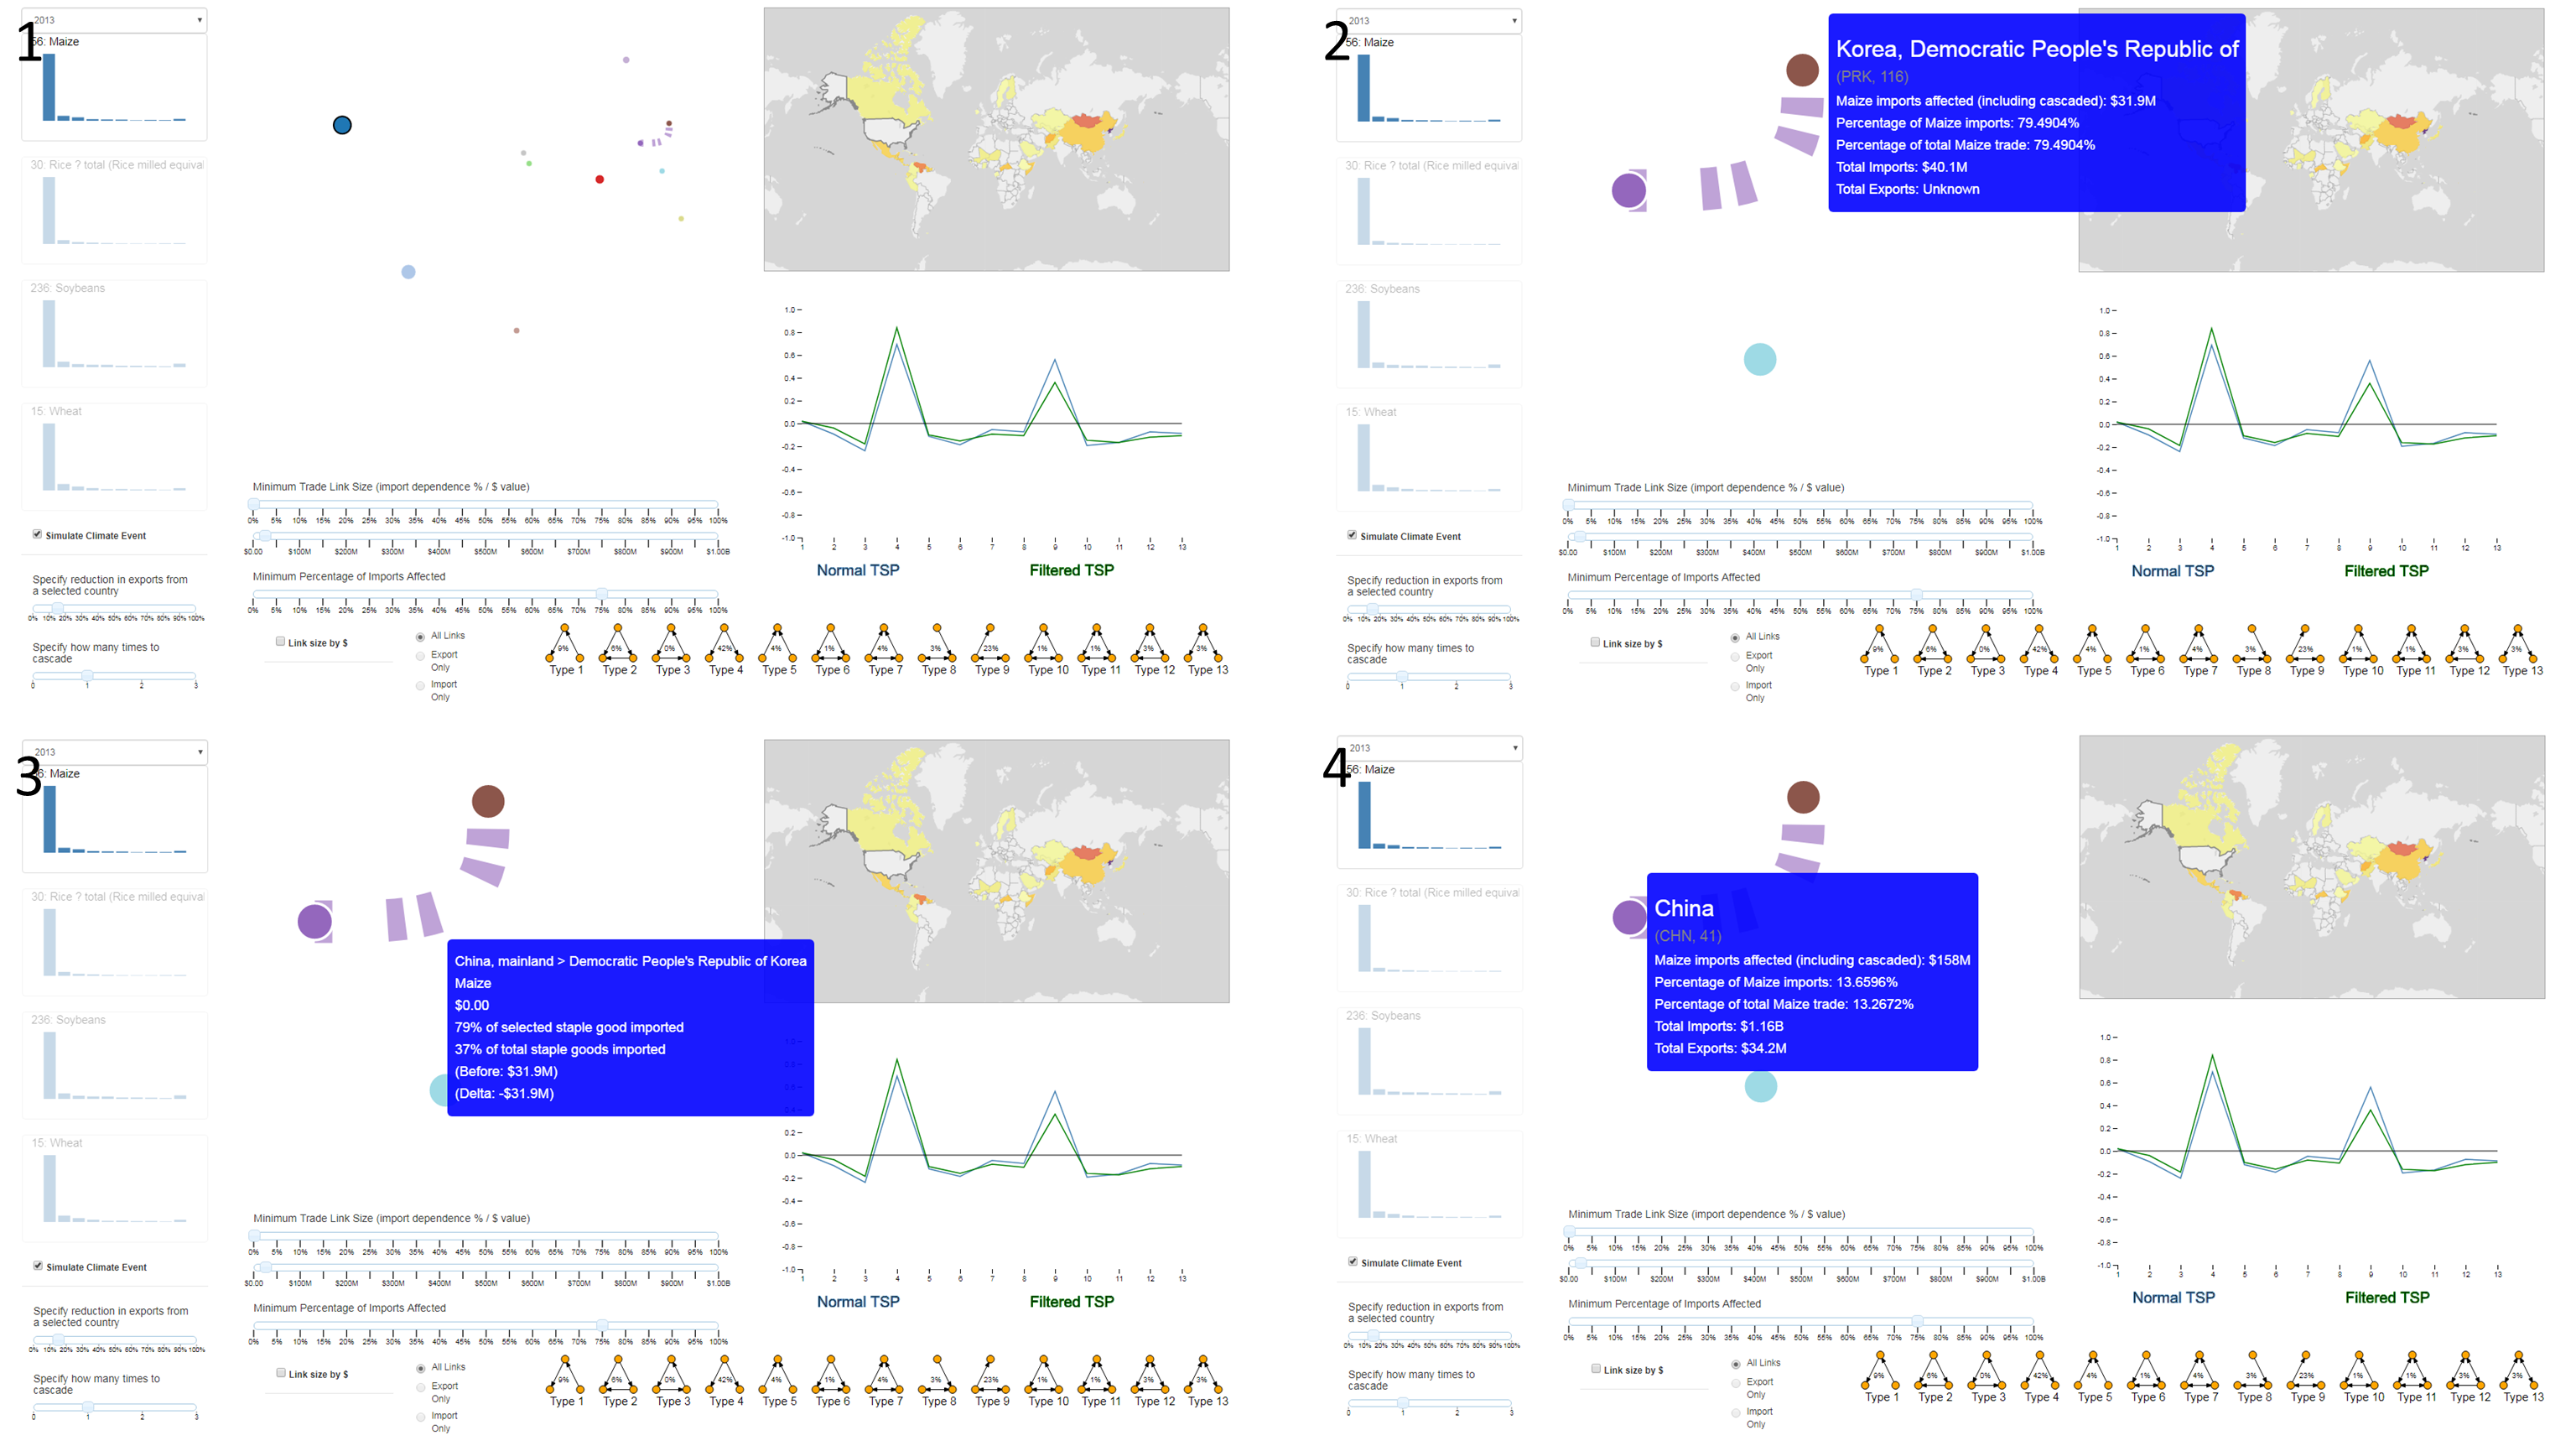
\includegraphics[width=\textwidth]{figures/cs2-4.png}}
	\caption[EXAMINING THE RESULTS OF A SIMULATION, FILTERED ON MODERATE DOLLAR VALUE (\$25 MILLION) AND LARGE IMPORT LOSSES (75\% LOSS)]{Examining the results of a simulation, filtered on moderate dollar value (\$25 million) and large import losses (75\% loss). 1: {Simulation results filtered on countries with import losses of at least 75\% and showing only links of at least a \$25 million dollar value}; 2: {Tooltip showing the impact to North Korea. The link is also drawn with alternating dashes and spaces, indicating it has been broken.}; 3: {Tooltip of the trade link from China to North Korea}; 4: {Tooltip showing the impact to China} }
	\label{cs2-4}
\end{figure}
This case study highlights the usefulness of these cascading, second-order effects. In the example of Venezuela we are able to see that Venezuela is more heavily affected than the direct trade link would suggest. In the example of North Korea there is no direct trade link and without cascading effects being accounted for, the vulnerability to North Korea may not be considered at all. The ability to visualize these links facilitates the identification of these potentially vulnerable, import reliant countries. This is even more apparent when those countries are dependent on a small number of suppliers as seen in both cases presented here.\par
